\documentclass[a4paper,12pt]{article}
\usepackage[utf8]{inputenc}

\usepackage[utf8]{inputenc}
\usepackage[T2A]{fontenc}
\usepackage[russian]{babel}
\usepackage{amsthm}
\usepackage{amsmath}
\usepackage{amssymb}
\usepackage{tikz}
\usepackage{textcomp}
\usepackage{marvosym}
\usepackage{ esint }
\setlength{\topmargin}{-0.5in}
\setlength{\textheight}{9.1in}
\setlength{\oddsidemargin}{-0.4in}
\setlength{\evensidemargin}{-0.4in}
\setlength{\textwidth}{7in}
\setlength{\parindent}{0ex}
\setlength{\parskip}{1ex}
\newcommand{\ndiv}{\hspace{-4pt}\not|\hspace{2pt}}
\usepackage{graphicx}
\usepackage{float}
\usepackage{wrapfig}
\usepackage{pgfplots}
\usepackage{caption}
\pgfplotsset{compat=1.16}

\title{Лабораторная работа № 3.1.3\\Измерение магнитного поля Земли}
\author{Илья Прамский}
\date{Сентябрь 2023}

\begin{document}

\maketitle
\newpage
\subsection*{1}
\vspace{5mm}
\section*{Введение}

\begin{flushleft}
  \textbf{Цель работы:} исследовать свойства постоянных неодиомвых магнитов, измерить с их помощью горизонтальную и вертикальную составляющие индукции магнитного поля Земли и магнитное наклонение.

\end{flushleft}

\begin{flushleft}
  \textbf{В работе используются:} неодимовые магниты; тонкая нить для изготовления крутильного маятника; медная проволока; электронные весы; секундомер; измеритель магнитной индукции; штангенциркуль; брусок, линейка и штатив из немагнитных материалов; набор гирь и разновесов.

\end{flushleft}

\section*{Теоретическая справка}

Простейший магнитный диполь может быть образован витком с током или постоянным магнитом. По определению, магнитный момент $\vec{\mathfrak{m}}$ тонкого витка площадью $S$ с током $I$ равен (в СИ)\[\vec{\mathfrak{m}}=I\vec{S},\].

Магнитное поле точечного диполя определяется по формуле, аналогичной формуле для поля элементарного электрического диполя:\[\vec{B}_{\text{дип}}=\frac{\mu_0}{4\pi}\left(\frac{3\left(\vec{\mathfrak{m}}\cdot\vec{r}\right)\vec{r}}{r^5}-\frac{\vec{\mathfrak{m}}}{r^3}\right).\]

Во внешнем магнитном поле с индукцией $\vec{B}$ на точечный магнитный диполь $\vec{\mathfrak{m}}$ действует механический момент сил\[\vec{\mathcal{M}}=\left[\vec{\mathfrak{m}}\times\vec{B}\right].\]При этом потенциальная энергия, которой обладает диполь с постоянным $\vec{\mathfrak{m}}$, равна\[W=-\left(\vec{\mathfrak{m}}\cdot\vec{B}\right).\]Когда диполь ориентирован вдоль внешнего поля ($\mathfrak{m}\parallel\vec{B}$), он находится в состоянии \textit{равновесия} ($\vec{\mathcal{M}}=0$). При этом \textit{устойчивым} будет только состояние, в котором диполь \textit{сонаправлен} с полем $\vec{\mathfrak{m}}\uparrow\uparrow\vec{B}$, поскольку его потенциальная энергия достигает \textit{минимума} $(W_{min}=-\mathfrak{m}B)$. При противоположной ориентации энергия будет иметь максимум $W_{max}=\mathfrak{m}B$, и состояние равновесия будет неустойчивым.

В \textit{неоднородном} внешнем поле выражение для энергии постоянного диполя сохраняется. При этом кроме момента сил на диполь действует ещё и сила\[\vec{F}=-\nabla W=\left(\vec{\mathfrak{m}}\cdot\nabla\right)\vec{B}.\]В частности, проекция этой силы на ось $x$ имеет вид\[F_x=\mathfrak{m}_x\frac{\partial B_x}{\partial x}+\mathfrak{m}_y\frac{\partial B_y}{\partial y}+\mathfrak{m}_z\frac{\partial B_z}{\partial z}.\]

Рассчитаем силу взаимодействия магнитов с моментами $\vec{\mathfrak{m}}_1$ и $\vec{\mathfrak{m}}_2$ в рамках модели точечных диполей. В частном случае, когда моменты двух небольших магнитов направлены вдоль соединяющей их прямой: $\vec{\mathfrak{m}}_{1,2}\parallel\vec{r}$, где $\vec{r}$ -- радиус-вектор между ними, магниты взаимодействуют с силой\[F_{12}=\mathfrak{m}_1\frac{\partial B_2}{\partial r}=\mathfrak{m}_1\frac{\partial\left(\frac{2\mathfrak{m}_2}{r^3}\right)}{\partial r}  \cdot \frac{\varphi_0}{4\pi} = -\frac{6\mathfrak{m}_1\mathfrak{m}_2}{r^4} \cdot \frac{\varphi_0}{4\pi}\]Здесь магниты притягиваются, если их магнитные моменты сонаправлены $(\vec{\mathfrak{m}}_1\uparrow\uparrow\vec{\mathfrak{m}}_2)$, и отталкиваются, если направлены противоположно $(\vec{\mathfrak{m}}_1\uparrow\downarrow\vec{\mathfrak{m}}_2)$.

Если магнитные моменты направлены перпендикулярно соединяющей их прямой: $\vec{\mathfrak{m}}_{1,2}\perp\vec{r}$, то нетрудно показать, что сила их взаимодействия окажется в два раза меньшей и будет иметь противоположный знак:\[F_{12}=\frac{3\mathfrak{m}_1\mathfrak{m}_2}{r^4}\ \text{(ед. СГС)}\](диполи притягиваются при $\vec{\mathfrak{m}}_1\uparrow\downarrow\vec{\mathfrak{m}}_2$ и отталкиваются при $\vec{\mathfrak{m}}_1\uparrow\uparrow\vec{\mathfrak{m}}_2$).

Магнитное поле однородно намагниченного шара радиусом $R$ может быть вычислено точно. На расстояниях $r\geq R$ от центра шара оно совпадает с полем точечного магнитного диполя, расположенного в центре, магнитный момент $\mathfrak{m}$ которого совпадает с полным моментом шара. Внутри шара магнитное поле однородно -- нетрудно получить, что при $r < R$\[\vec{B}_0=\frac{\mu_0\vec{\mathfrak{m}}}{2\pi R^3}\ \left[\text{СИ}\right].\]

В качестве ещё одной характеристики материала магнита используют остаточную \textit{намагниченность} $\vec{M}$. По определению, намагниченность равна \textit{объёмной плотности магнитного момента}, поэтому для однородно намагниченного шара\[\vec{\mathfrak{m}}=\vec{M}V,\]где $V=\frac{4\pi}{3}R^3$ -- объём магнита. Величину $\vec{B}_r=\mu_0\vec{M}$ называют \textit{остаточной индукцией} материала.

Нетрудно видеть, что индукция $\vec{B}_p$ \textit{на полюсах} однородно намагниченного шара неправлена по нормали к поверхности и совпадает поэтому с индукцией внутри шара: $\vec{B}_p=\vec{B}_0$. Тогда величина $B_p$ связана с остаточной индукцией $B_r$ соотношением\[B_p=B_0=\frac{2}{3}B_r.\]
\newpage
\section*{Экспериментальная установка}

\subsection*{Определение величины магнитного момента шариков}

Величину магнитного момента $\mathfrak{m}$ одинаковых шариков можно рассчитать, зная их массу $m$ и определив максимальное расстояние $r_{max}$, на котором они ещё удерживают друг друга в поле тяжести. При максимальном расстоянии сила тяжести шариков равна силе их магнитного притяжения:\[\frac{6\mathfrak{m}^2}{r_{max}^4}  \cdot \frac{\varphi_0}{4\pi} = mg\implies\mathfrak{m}=\sqrt{\frac{mgr_{max}^4 \cdot 4\pi}{6 \cdot \varphi_0}}.\]

По величине магнитного момента $\mathfrak{m}$ можно рассчитать величину индукции магнитного поля вблизи любой точки на поверхности шара радиуса $R$. Максимальная величина индукции наблюдается на полюсах:\[\vec{B}_p=\frac{2\vec{\mathfrak{m}}}{R^3}.\]

Величину магнитного момента шариков можно определить макже по силе их сцепления. Она определяется как сила, необходимая для разрыва двух сцепившихся магнитных шариков. Сила сцепления максимальна, если шары соединяются своими противоположными полюсами.

Максимальную силу сцепления можно определить по весу магнитной цепочки, которую способен удержать самый верхний магнитный шарик. Если цепь состоит из одинаковых магнитных шариков, то при определённой длине она она оторвётся от верхнего шарика. Приэтом, учитывая, что сила приятжения убывает как $F\sim\frac{1}{r^4}$, для расчёта прочности цепочки достаточно учитывать силу взаимодействия верхенего шара с тремя-четырьмя ближайшими соседями.

Если сила сцепления двух одинаковых шаров диаметром $d$ с магнитными моментами $\mathfrak{m}$ равна\[F_0=\frac{6\mathfrak{m}^2}{d^4}  \cdot \frac{\varphi_0}{4\pi} ,\]то минимальный вес цепочки, при которой она оторвётся от верхнего шарика, равен\[F=F_0\sum_{n=1}^{+\infty}\frac{1}{n^4}=\frac{\pi^4}{90}F_0\approx1,08F_0.\]

Таким образом, сила сцепления двух шаров равна\[F_0=\frac{90}{\pi^4}F=0,924F.\]
\newpage
\subsection*{Измерение горизонтальной составляющей индукции магнитного поля Земли}

Магнитное поле в настоящей работе определяется по периоду крутильных колебаний магнитной стрелки вокруг вертикальной оси.

\begin{wrapfigure}{r}{5cm}
	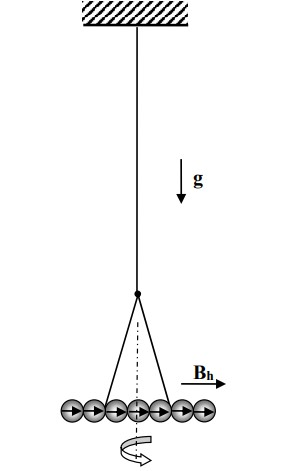
\includegraphics[width=5cm]{horizont.jpg}
	\caption{Крутильный маятник}
	\label{mahovik}
\end{wrapfigure}

"Магнитная стрелка" образована из сцепленных друг с другом противоложными полюсами шариков и с помощью $\Lambda$-образного подвеса подвешена в горизонтальном положении. Магнитные моменты шариков направлены в одну сторону вдоль оси "стрелки". Под действием вращательного момента $\vec{M}=\vec{\mathfrak{m}}_0\times\vec{B}$ магнитный момент "стрелки" $\vec{\mathfrak{m}}_0$ выстроится вдоль горизонтальной составляющей магнитного поля Земли $\vec{B}_h$ в направлении $S\to N$. При отклонении "стрелки" на угол $\theta$ от равновесного положения в горизонтальной плоскости возникают крутильные колебания вокруг вертикальной оси, проходящей через середину "стрелки". Если пренебречь упругостью нити, то уравнение крутильных колебаний такого маятника при малых амплитудах ($\sin{\theta}\approx\theta$) имеет вид\[I_n\ddot{\theta}+\mathfrak{m}_0B_h\theta=0,\]где $I_n=\frac{1}{12}m_{\text{ст}}l_{\text{ст}}^2=\frac{1}{12}n^3md^2$ -- момент инерции "стрелки" , состоящей из $n$ шариков, который можно с хорошей точностью приблизить моментом инерции тонкого однородного стержня соответствующей массы и длины, а $\mathfrak{m}_0=n\mathfrak{m}$ -- полный магнитный момент стрелки.

Таким образом, период колебаний маятника оказывается равен\[T(n)=2\pi\sqrt{\frac{md^2}{3\mathfrak{m}B_h}}n=kn,\]где $k=2\pi\sqrt{\frac{md^2}{3\mathfrak{m}B_h}}$.

\subsection*{Измерение вертикальной составляющей индукции магнитного поля Земли. Магнитное наклонение.}

Для измерения вертикальной составляющей $B_v$ вектора индукции поля Земли используется та же установка, что и для измерения горизонтальной составляющей с тем лишь отличием, что магнитная "стрелка" подвешивается на нити без $\Lambda$-образного подвеса. В этом случае магнитная "стрелка" , составленная из чётного числа шариков и подвешенная на тонкой нити за середину, расположится не горизонтально, а под некоторым отличным от нуля углом к горизонту. Это связано с тем, что вектор $\vec{B}$ индукции магнитного поля Земли в общем случае не горизонтален, а образует с горизонтом угол $\beta$, зависящий от географической широты $\varphi$ места, где проводится опыт. Величина угла $\beta$ называется магнитным наклонением.

\begin{wrapfigure}{r}{5cm}
	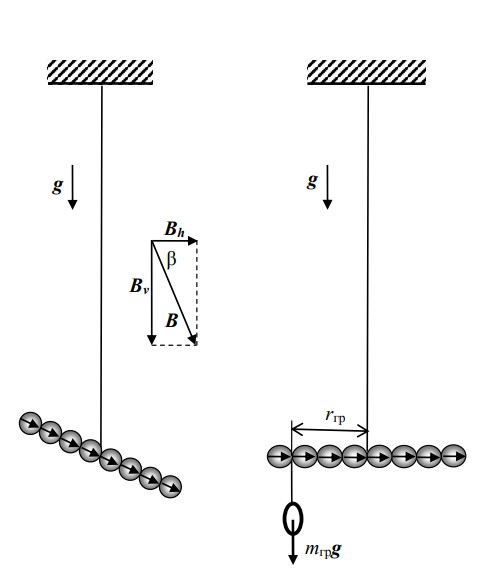
\includegraphics[width=5cm]{vert.jpg}
	\caption{Определение вертикальной составляющей магнитного поля Земли}
	\label{mahovik}
\end{wrapfigure}

С помощью небольшого дополнительного грузика "стрелку" можно "выровнять" , расположив её горизонтально. В этом случае момент силы тяжести груза относительно точки подвеса будет равен моменту сил, действующих на "стрелку" со стороны магнитного поля. Если масса уравновешивающего груза равна $m_{\text{гр}}$, плечо силы тяжести $r_{\text{гр}}$, а полный магнитный момент "стрелки" $\mathfrak{m}_0=n\mathfrak{m}$, то в равновесии\[m_{\text{гр}}gr_{\text{гр}}=n\mathfrak{m}B_v,\]где $B_v$ -- вертикальная составляющая поля Земли. Видно, что момент $M(n)$ силы тяжести уравновешивающего груза пропорционален числу $n$ шариков, образующих магнитную "стрелку" :\[M(n)=An,\]где $A=\mathfrak{m}B_v$.

\section*{Ход работы}
\subsection*{Определение магнитного момента, намагниченности и остаточной магнитной индукции вещества магнитных шариков}
1. Для начала измерим диаметр и массу шариков при помощи штангенциркуля и электронных весов соответственно.

Получается $d_{\text{ш}} = 0,59 \pm 0,01$см, $\langle m_{\text{ш}} \rangle = 0,837 \pm 0,001$ г.

Теперь при помощи магнетометра измерим индукцию поля $B_{\text{р}}$ на полюсах шарика.

Получается $B_{\text{р}} = 231$ мТл.

2. Далее пользуясь методом A(измерение максимального расстояние между шариками, при котором они удерживают друг друга в поле тяжести Земли), рассчитаем величину магнитного момента шарика. На опыте получилось, что расстояние между шариками не может быть больше $r = 1,60 \pm 0,01$ см.

Тогда $r_{max} = r + 2 \cdot \frac{d_{\text{ш}}}{2} = 2,190 \pm 0,017$ см.

Вычисляя момент шарика по формуле метода A, получаем $\textsf{m} = 0,0559 \pm 0,0008 A \cdot \text{м}^2$ 

3. Теперь, пользуясь методом Б, рассчитаем силу сцепления двух шаров и определим по ней магнитный момент шарика.

При взятии цепи из 25 шариков, минимальный масса системы цепочки с гирей равна $m_{min} = 245,270 \pm 0,001$ г.

Тогда сила сцепления двух шаров равна $F_0 = \frac{F}{1,08}$, где $F = m_{min} \cdot g$. Получается $F_0 = 2,23$ Н.

Магнитный момент шарика равен $\textsf{m} = 0,067 \pm 0,002 A \cdot \text{м}^2$.

Видно, что значения, полученные двумя методами, отличаются друг от друга. Хоть первый метод и дал погрешность меньшую, чем второй, многие неточности(такие как постоянное придерживание шариков в первом методе, движение немагнитного бруска между шариками) были неучтены в первом методе, из-за чего он дает менее точный результат, поэтому при дальнейших расчетах будем пользоваться результатом метода Б.

4. Рассчитаем величину намагниченности материала шариков M и остаточной индукции магнитного поля $B_r$:
\[\textsf{m} = M \cdot V \Rightarrow M = \frac{\textsf{m}}{V} = \frac{\textsf{m}}{\frac{4}{3} \cdot \pi \cdot {(\frac{d}{2})}^3}\]
$M = 623362 \pm 36754 A \cdot \text{м}^{-1}$

Тогда $B_r = \varphi_0 \cdot M = 0,78 \pm 0,05$ Тл.

Получившееся значение меньше справочного(1,22 Тл). Это может быть связано с постепенным размагничиванием шариков из-за механического воздействия.

5. Теперь рассчитаем индукцию у полюсов шарика. Получается $B_r = 0,52 \pm 0,03$ Тл. Видно, что значение у полюсов отличается от расчитанного. Это можно объяснить тем, что при измерении поля шариков при помощи магнитометра, его было сложно установить к полюсам на длительное время, из-за чего значение, полученное экспериментально, меньше полученного при расчетах.

\subsection*{Определение горизонтальной составляющей магнитного поля Земли}
1. Для начала соберем кольцо из шариков и рассмотрим его колебания(в данном случае магнитный момент этого маятника будет равен нулю, а значит колебания будут создаваться под воздействием упругости нити). Получилось: $t = 41,12$ с при $5$ колебаниях, а значит период равен $T = 8,224$ с, что в несколько раз больше характерного периода колебаний прямой стрелки, из-за чего можно считать, что упругость нити можно не учитывать.

2. Теперь рассмотрим зависимость периода колебаний прямой стрелки из шариков в зависимости от их количества в ней.

\begin{center}
  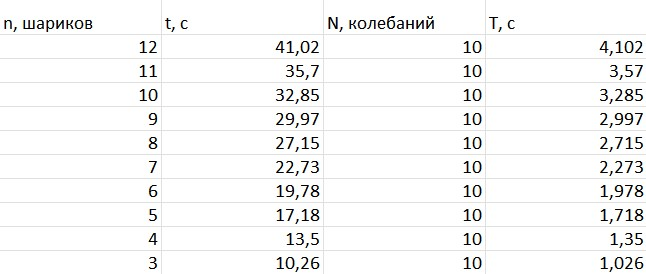
\includegraphics[scale=1.2]{tabliza.jpg}
  \label{fig:picture}
\end{center}

\newpage
По данным из таблицы построим график зависимости $T(n)$. Из него видно, что зависимость линейная. По методу наименьших квадратов найдем значение коэффициента пропорциональности и проведем прямую.

\begin{center}
  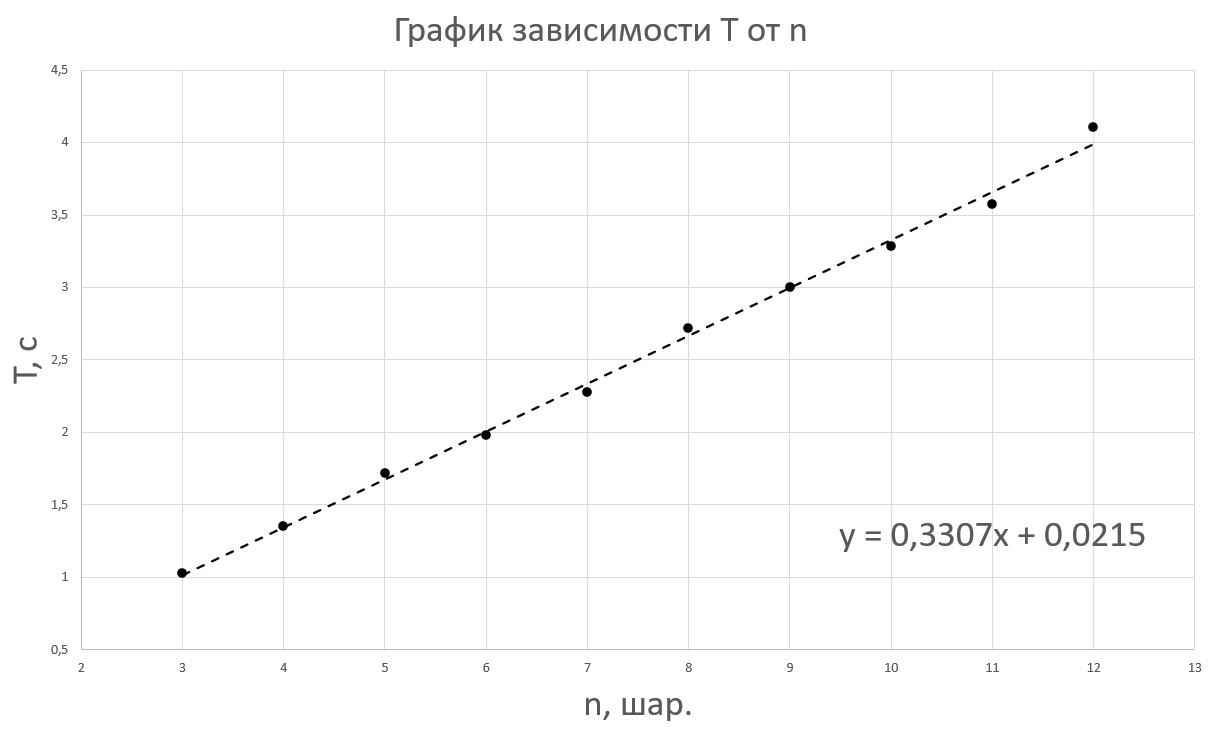
\includegraphics[scale=0.7]{graphik.jpg}
  \label{fig:picture}
\end{center}

Зная чему равен коэффициент пропорциональности($k = 0,331 \pm 0,007 c$), найдем значение горизонтальной составляющей магнитного поля Земли.
\[k = 2 \cdot \pi \cdot \sqrt{\frac{m \cdot R^2}{3 \cdot \textsf{m} \cdot B_{\parallel}}}\]
$B_{\parallel} = 1,30 \pm 0,08 \cdot 10^{-5}$ Тл.

\subsection*{Определение вертикальной составляющей магнитного поля Земли}
1. Для стрелки, подвешанной за середину с помощью нити, измерим массу груза, необходимую для уравновешения стрелки в горизонтальное положение. Узнав эту массу, измерим момент силы тяжести, и из условия равновесия приравняем его к механическому моменту магнитного поля Земли. Проделаем вышесказанное для стрелок с разным четным количеством шариков.

Здесь $r_{\text{гр}}$ - расстояние от точки подвеса стрелки до точки подвеса уравновешивающего груза; 

\begin{center}
  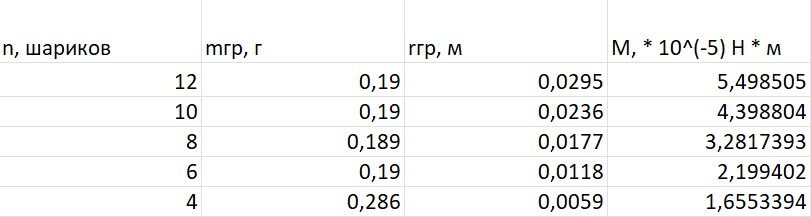
\includegraphics[scale=0.7]{tabliza2.jpg}
  \label{fig:picture}
\end{center}

По данным из таблицы построим график зависимости M(n).

\begin{center}
  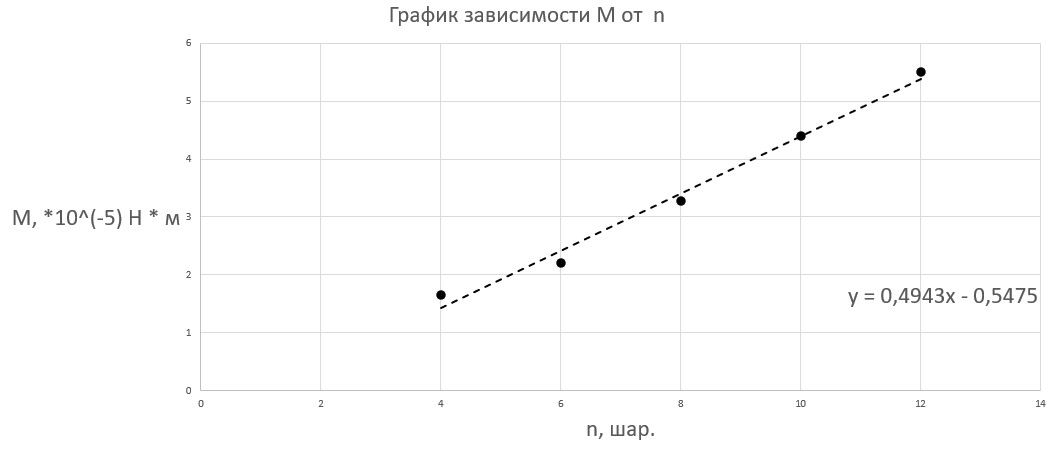
\includegraphics[scale=0.7]{graphik2.jpg}
  \label{fig:picture}
\end{center}

По методу наименьших квадратов найдем коэффициент пропорциональности и изобразим прямую на графике. Из формулы видно, что в данном случае коэффициент пропорциональности равен $k = \textsf{m} \cdot B_{v}$.

Получается $k = 0,49 \pm 0,03 \cdot 10^{-5} H \cdot \text{м}^2$. 

Тогда вертикальная составляющая магнитного поля равна
\[B_v = \frac{k}{\textsf{m}} = 74 \pm 5 \text{мкТл.}\]

В итоге магнитное наклонение равно $\beta = \arctan{\frac{B_v}{B_\parallel}} = 80^{\circ}$. Общее магнитное поле Земли $B = 75 \pm 5$ мкТл.

\section*{Вывод}
В ходе данной работы были исследованный свойства неодимых магнитов, измерены их магнитные моменты при помощи нескольких методов; также были получены с помощью этих магнитов значения вертикальной и горизонтальной составляющей индукции магнитного поля Земли. Хоть и горизонтальная составляющая была близка к справочной($B_{\parallel} =  15-20$ мкТл), однако вертикальная часть пусть и не на порядок, но достаточно сильно отличается от справочной(получено $B_v = 74$ мкТл, табличное значение $B_v = 46$ мкТл). Это можно объяснить тем, что вокруг экспериментальной установки находились другие приборы, которые могли своим полем изменить это значение(подтверждением этого является сдвиг стрелки в противоположную от севера сторону в одной части аудитории, и правильное направление стрелки в другой части).

\end{document}